\graphicspath{{./figs/}}
\newcommand{\norm}[1]{\left\lVert#1\right\rVert}
\section{Постановка задачи}

Моделируется нейтронное поле в многогрупповом диффузионном приближении. Динамика нейтронов 
рассматривается в ограниченной выпуклой двумерной или трехмерной области  $\Omega$ ($\bm x = \{x_1, ..., x_d\} \in \Omega, \ d = 2,3$) с границей $\partial \Omega$. Перенос нейтронов описывается системой уравнений
\begin{equation}\label{1}
\begin{split}
 \frac{1}{v_g} \frac{\partial \phi_g}{\partial t} - & \nabla \cdot D_g \nabla \phi_g + \Sigma_g \phi_g 
 - \sum_{g\neq g'=1}^{G} \Sigma_{s,g'\rightarrow g} \phi_{g'} \\
 =  & \ (1-\beta) \chi_g \sum_{g'=1}^{G} \nu \Sigma_{fg'} \phi_{g'} + \widetilde{\chi}_g \sum_{m=1}^{M} \lambda_m c_m , \quad 
 g = 1,2, ..., G .
\end{split}
\end{equation} 
Здесь $\phi_g(\bm x,t)$ --- поток нейтронов группы $g$ в точке $\bm x$ на момент времени $t$,
$G$ --- число групп,
$v_g$ --- эффективная скорость нейтронов в группе $g$,
$D_g(\bm x)$ --- коэффициент диффузии, $\Sigma_g(\bm x,t)$ --- сечение поглощения,
$\Sigma_{s,g'\rightarrow g}(\bm x,t)$ --- сечение рассеяния с группы $g'$ в группу $g$,
$\beta$ --- эффективная доля запаздывающих нейтронов, $\chi_g$, $\widetilde{\chi}_g$  --- спектры мгновенных и запаздывающих нейтронов, 
$\nu\Sigma_{fg}(\bm x,t)$ --- сечение генерации группы $g$,
$c_m$ --- плотность источников запаздывающих нейтронов $m$ типа,  $\lambda_m$ --- постоянная распада источников запаздывающих нейтронов,
$M$ --- число типов запаздывающих нейтронов.
Плотность источников запаздывающих нейтронов описывается уравнениями
\begin{equation}\label{2}
 \frac{\partial c_m}{\partial t} + \lambda_m c_m = \beta_m \sum_{g=1}^{G} \nu \Sigma_{fg} \phi_g,
 \quad m = 1,2, ..., M, 
\end{equation} 
где $\beta_m$ --- доля запаздывающих нейтронов  $m$ типа, причем
\[
 \beta = \sum_{m=1}^{M} \beta_m .
\] 
На границе области $\partial \Omega$ ставятся условия альбедного типа:
\begin{equation}\label{3}
 D_g\frac{\partial \Phi_g}{\partial n} + \gamma_g \Phi_g = 0, \quad 
 \quad g = 1,2, ..., G ,
\end{equation}
где $n$ --- внешняя нормаль к границе $\partial \Omega$.
\\
Рассматривается задача для системы уравнений (\ref{1}), (\ref{2}) с краевыми условиями(\ref{3}), и начальными условиями:
\begin{equation}\label{4}
 \phi_g(\bm x,0) = \phi_g^0(\bm x), 
  \quad  g = 1,2, ..., G .
\end{equation} 
Запишем краевую задачу (\ref{1}), (\ref{2}), (\ref{3}), (\ref{4}) в операторной форме. 
Определим векторы $\bm \phi = \{\phi_1, \phi_2, ..., \phi_G\}$, $\bm c = \{c_1, c_2, ..., c_M\}$ и матрицы
\[
 V = (v_{g g'}),
 \quad v_{g g'} = \delta_{g g'} v_g^{-1},
\] 
\[
 D = (d_{g g'}),
 \quad d_{g g'} = - \delta_{g g'} \nabla \cdot D_g \nabla,
\] 
\[
 S = (s_{g g'}),
 \quad  s_{g g'} =  \delta_{g g'} \Sigma_g - \Sigma_{s,g'\rightarrow g} ,
\] 
\[
 R = (r_{g g'}),
 \quad  r_{g g'} = (1-\beta)\chi_g \nu \Sigma_{fg'} ,
\] 
\[
 B = (b_{g m}),
 \quad b_{g m} = \widetilde{\chi}_g \lambda_m,
\] 
\[
 \Lambda = (\lambda_{m m'}),
 \quad  \lambda_{m m'} = \lambda_m \delta_{m m'} ,
\] 
\[
 Q = (q_{mg}),
 \quad  q_{mg} = \beta_m \nu \Sigma_{fg},
\]
\[
 \quad g, g' = 1,2, ..., G,
 \quad m, m' = 1,2, ....,M,  
\]
где
\[
 \delta_{g g'} = \left \{ 
 \begin{matrix}
 1, & g = g', \\
 0, & g \neq  g',
 \end{matrix}
 \right . 
\] 
есть символ Кронеккера.
Будем работать на множестве векторов $\bm \phi$, компоненты которого удовлетворяют граничным условиям 
(\ref{3}). С учетом введенных обозначений система уравнений (\ref{1}), (\ref{2}) записывается в следующем виде
\begin{equation}\label{5}
\begin{split}
V \frac{d \bm \phi}{d t} + (D+S) \bm \phi &= R \bm \phi + B\bm c,
\\
\frac{d \bm c}{d t} + \Lambda \bm c &= Q \bm \phi. 
\end{split}
\end{equation}  
Для (\ref{5}) рассматривается задача Коши, когда
\begin{equation}\label{6}
 \bm \phi(0) = \bm \phi^0,
\end{equation} 
где $\bm \phi^0 = \{ \phi_1^0,  \phi_2^0, ...,  \phi_G^0 \}$.

\section{Спектральная задача} 

Для характеристики динамических процессов в ядерном реакторе, которые описываются задачей Коши 
(\ref{5}), (\ref{6}) привлекаются решения некоторых спектральных задач \cite{Bell1970,hetrick1971dynamics,stacey}.

Обычно рассматривается спектральная задача
\begin{equation}\label{s1}
\begin{split}
(D+S) \bm \varphi  &= \lambda^{(k)}(R \bm \varphi + B \bm s),\\
\Lambda \bm s &= \lambda^{(k)} Q \bm \varphi.
\end{split}
\end{equation} 
Это задача (\ref{s1}) известно как Lambda modes спектральная задача. 
Для характеристики нейтронного поля привлекается минимальное собственное значение, так что
\[
 k = \frac{1}{\lambda^{(k)}_1}  
\] 
есть эффективный коэффициент размножения.
Значение $k = \lambda^{(k)}_1 = 1$ связывается с критическим состоянием реактора, соответствующая
собственная функция $\varphi_1(\bm x)$ есть стационарное решение уравнения (\ref{5}).
При $k > 1$  говорят о надкритическом состоянии реактора, при $k < 1$  --- о подкритическом состоянии.

%В силу несамосопряженности операторов нейтронного переноса мы имеем, вообще говоря,
%комплексные собственные значения. 
%Для главного собственного значения свойство действительности и положительности 
%собственного значения для системы уравнений нейтроники  доказывается на основе принципа максимума при некоторых ограничениях 
%на коэффициенты операторов переноса нейтронов \cite{habetler1961existence}. 
%Это касается также и несамосопряженного эллиптического оператора второго порядка \cite{bookEvans}. 

Спектральную задачу (\ref{s1}) нельзя напрямую связать с динамическими процессами в ядерном реакторе.
В лучшем случае мы можем выделить только предельный случай --- стационарное критическое состояние.
Более приемлемая спектральная характеристика для нестационарного уравнения (\ref{5}) связана со спектральной задачей 
\begin{equation}\label{s2}
\begin{split}
 (D+S - R) \bm \varphi  -  B \bm s & = \lambda^{(\alpha)} V \bm \varphi , \\
 \Lambda \bm s - Q \bm \varphi & =  \lambda^{(\alpha)}   \bm s .
\end{split} 
\end{equation} 
Фундаментальное собственное значение
\[ 
 \alpha = \lambda^{(\alpha)}_1
\]
называется \cite{Bell1970}
$\alpha$--eigenvalues или period eigenvalues.
С собственным значением $\alpha$ 
можно связать асимптотическое поведение
решения задачи Коши (\ref{5}), (\ref{6}) при больших временах.
В этом регулярном режиме поведение реактора описывается функцией $e^{-\alpha t} \varphi_1(\bm x)$.


\section{Аппроксимация по времени}
\label{s-3}
Для численного решения задачи методом конечных элементов, необходимо дискретизировать производные по времени используя конечно-разностные схемы, а затем каждую стационарную задачу привести к вариационной постановке \cite{hebert}.\\
Для аппроксимации по времени рассмотрим две схемы: чисто-неявную, явно-неявную. Пусть $\tau$ шаг  равномерной сетки по времени, такой что $\bm\phi^{n}=\bm\phi(\bm x,t_n)$, $\bm c^n=\bm c(\bm x, t_n)$ где $t_n=n\tau$, $n=0,1,...,N$, $N\tau=T$.  \\
Проинтегрируем уравнение (\ref{2}) от $t_{n}$ до $t_{n+1}$, тогда
\begin{align}\label{at0}
c_m^{n+1} = c_m^n e^{-\lambda_m\tau} + \beta_m e^{-\lambda_m\tau}\int_{t_n}^{t_{n+1}}e^{\lambda_m (t-t_n)} \sum_{g=1}^{G} \nu \Sigma_{fg} \phi_g,
 \quad m = 1,2, ..., M.
\end{align}
Рассмотрим для уравнения \ref{5} чисто-неявную разностную схему. Будем использовать верхную сумму для вычисления подынтегральной функции (\ref{at0}), тогда получаем
\begin{align}\label{at1}
\begin{split}
V \frac{\bm\phi^{n+1}-\bm\phi^n}{\tau}+(D+S) 
\bm \phi^{n+1} &= R \bm \phi^{n+1} + B\bm c^{n+1},
\\
\bm{c}^{n+1} & = \hat{\Lambda}\bm{c}^{n} + \tau Q \bm{\phi}^{n+1},
\end{split}
\end{align}
где
\[
\hat{\Lambda} = (\hat{\lambda}_{mm'}), \quad \hat{\lambda}_{mm'} = \delta_{mm'} e^{-\lambda_m\tau}
\]
Теперь рассмотрим для уравнения \ref{5} явно-неявную разностную схему. Для этого случая использовуем нижную сумму для вычисления подынтегральной функции (\ref{at0}), тогда получаем
\begin{align}\label{at2}
\begin{split}
V \frac{\bm{\phi}^{n+1} - \bm{\phi}^{n}}{\tau}+(D+S)\bm{\phi}^{n+1} &= R\bm{\phi}^{n} + B\bm{c}^{n+1} \\
\bm{c}^{n+1} & = \hat{\Lambda}\bm{c}^{n} + \tau \hat{Q} \bm{\phi}^{n},
\end{split}
\end{align}
где 
\[
\hat{Q} = (\hat{q}_{mg}), \quad \hat{q}_{mg}=e^{-\lambda_m\tau}\beta_m\nu\Sigma_{fg}
\]
Подставляем $\bm{c}^{n+1}$ из нижнего уравнения в верхнее 
 и перепишем так, чтобы $\bm\phi^{n+1}$ были с левой стороны уравнения, а $\bm\phi^{n}$ с правой стороны уравнения, тогда получаем СЛАУ
\[
A u = b,
\]
где $u = \bm\phi^{n+1}$. Для уравнения (\ref{at1}) имеем
\[
A = \frac{V}{\tau}+D+S-R-\tau Q,\quad
b = \frac{V}{\tau}\bm\phi^n + \hat\Lambda \bm c^n.
\]
А для уравнения (\ref{at2}) имеем
\[
A = \frac{V}{\tau}+D+S, \quad
b = \left(\frac{V}{\tau}+R+\tau \hat Q\right)\bm\phi^n + \hat\Lambda \bm c^n.
\]

\section{Модельная задача}
Рассматривается тестовая задача для реактора ВВЭР-1000 без отражателя \cite{chao} в двумерном приближении 
($\Omega$ --- сечение активной зоны реактора). 
Геометрическая модель активной зоны ВВЭР-1000 состоит из набора кассет гексагональной формы
и представлена на рис.\ref{fig:1}, где цифрами показаны кассеты различных типов.
Размер кассеты «под ключ» равен 23.6 см. Диффузионные нейтронно-физические константы в системе измерений
СИ приведены в табл.\ref{t-1}. 
Используются граничные условия (\ref{3}) при задании $\gamma_g = 0.5, \ g = 1,2$. Задача рассматривается при $v_1 = 12 500 000$, $v_2 = 250 000$, $\lambda_1 = 0.08$ и $\beta_1 = 0.0065$.

\begin{figure}[htp]
  \begin{center}
    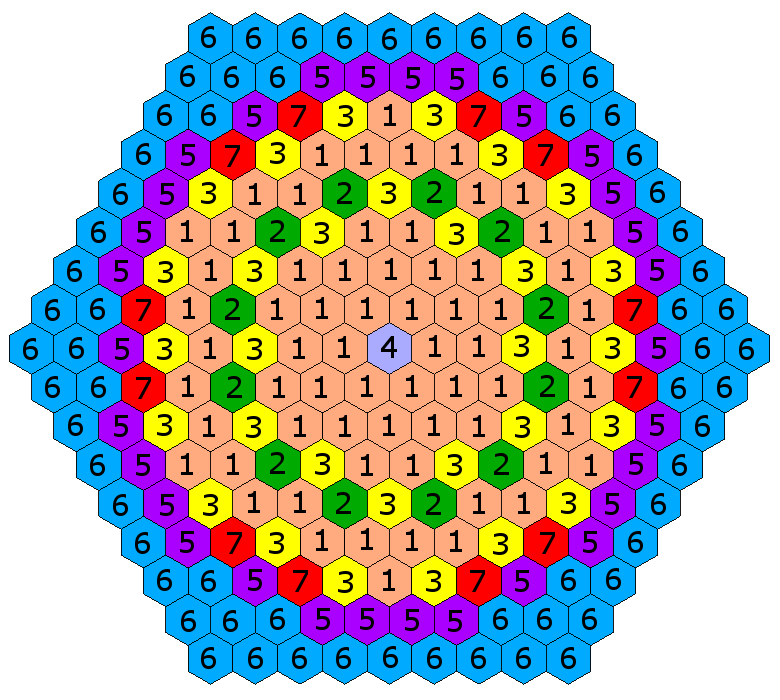
\includegraphics[width=0.75\linewidth] {1.png}
	\caption{Геометрическая модель активной зоны реактор ВВЭР-1000.}
	\label{fig:1}
  \end{center}
\end{figure} 

\begin{table}[htp]
\caption{Диффузионные константы для ВВЭР-1000}
\label{t-1}
\begin{center}
\begin{tabular}{|c|c|c|c|c|c|}
\hline
Материал & 1 & 2 & 3 & 4 & 5\\
\hline
$D_1$ & 1.38320e-0 & 1.38299e-0  & 1.39522e-0  & 1.39446e-0  & 1.39506e-0 \\
$D_2$ & 3.86277e-1 & 3.89403e-1 & 3.86225e-1 & 3.87723e-1 & 3.84492e-1 \\
$\Sigma_1 + \Sigma_{s,1\rightarrow 2}$ & 2.48836e-2 & 2.62865e-2 & 2.45662e-2 & 2.60117e-2 & 2.46141e-2\\
$\Sigma_2$ & 6.73049e-2 & 8.10328e-2 & 8.44801e-1 & 9.89671e-2 & 8.93878e-2\\
$\Sigma_{s,1\rightarrow 2}$ & 1.64977e-2 & 1.47315e-2 & 1.56219e-2 & 1.40185e-2 & 1.54981e-2\\
$\nu\Sigma_{f1}$ & 4.81619e-3 & 4.66953e-3 & 6.04889e-3 & 5.91507e-3 & 6.40256e-3\\
$\nu\Sigma_{f2}$ & 8.46154e-2 & 8.52264e-2 & 1.19428e-1 & 1.20497e-1 & 1.29281e-1\\
\hline
\end{tabular}
\end{center}
\end{table}

Для приближенного решение задачи используется метод конечных элементов \cite{quarteroni} 
на треугольных расчетных сетках. Число треугольников на одну кассету $\kappa=6, 24, 96$ (рис.\ref{fig:2}).
Используются стандартные лагранжевые конечные элементы степени $p=1, 2, 3$ (рис \ref{fig:fem}).
Программное обеспечение написано с использованием библиотеки инженерных и научных вычислений
FEniCS \cite{fenics}. Для численного решения спектральных задач привлекается SLEPc \cite{slepc}.
 
%Число треугольников на одну кассету $\kappa$  варьируется от 6 до 96 (рис.\ref{fig:2}).
%Используются стандартные лагранжевые конечные элементы степени $p=1,2,3$ (рис \ref{fig:fem}).

\begin{figure}[H]
  \begin{center}
\begin{minipage}{0.30\linewidth}
\center{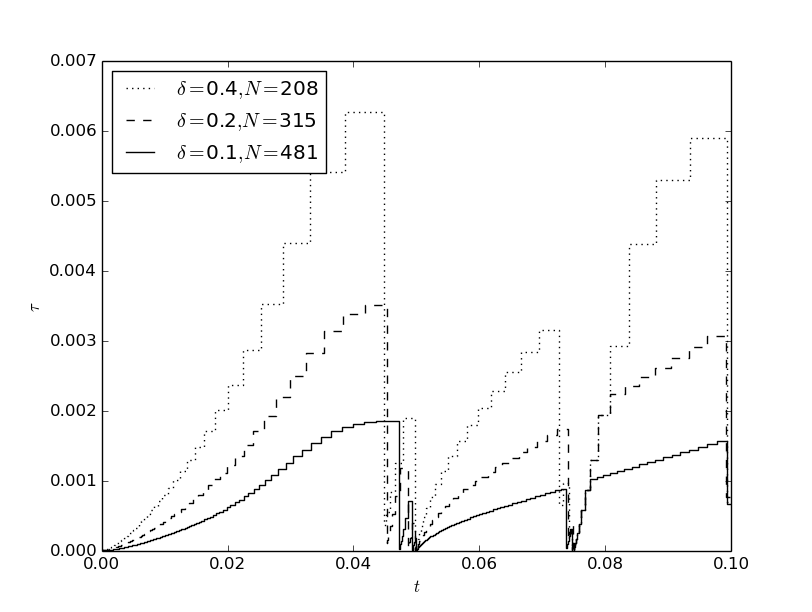
\includegraphics[width=1\linewidth]{2-1.png}}\\
\end{minipage}
\hfill
\begin{minipage}{0.30\linewidth}
\center{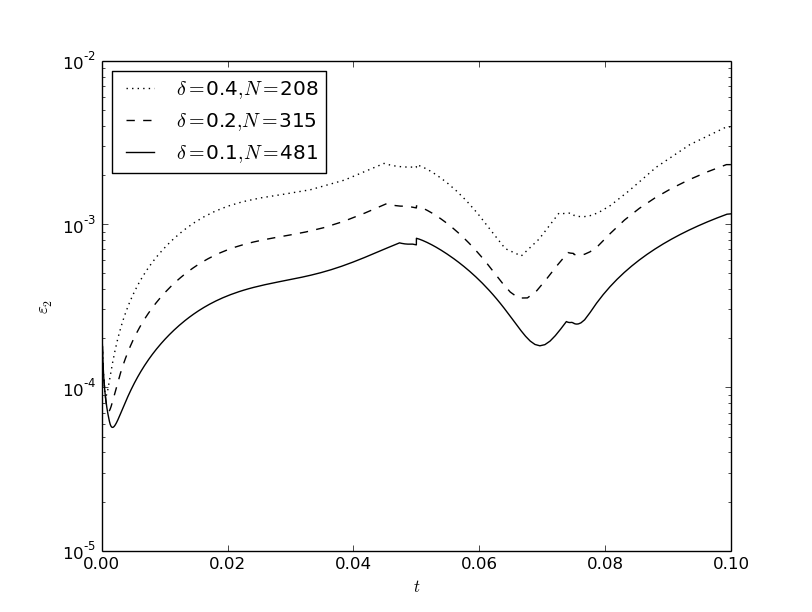
\includegraphics[width=1\linewidth]{2-2.png}}\\
\end{minipage}
\hfill
\begin{minipage}{0.30\linewidth}
\center{\includegraphics[width=1\linewidth]{2-3.png}}\\
\end{minipage}
\caption{Разбиение кассеты на 6, 24 и 96 конечных элементов.}
\label{fig:2}
  \end{center}
\end{figure}

\begin{figure}[htp]
  \begin{center}
    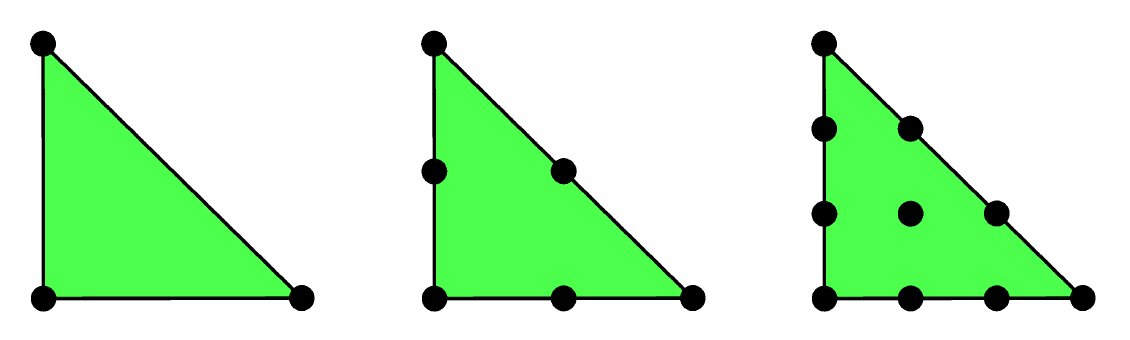
\includegraphics[width=1\linewidth] {fem.png}
	\caption{Лагранжевые полиномы 1, 2, 3 степени соответственно.}
	\label{fig:fem}
  \end{center}
\end{figure} 

\subsection{Решение Alpha Modes спектральной задачи}
%Следовательно со временем все высшие гармоники устоканяться и останется только одна. Если отнормировать решение спектральной задачи и решение нестационарной задачи, то со временем они должны сходится. 

Приведем результаты численного решения спектральной задачи (\ref{s2}).
В рамках используемого двухгруппового приближения имеем 
\begin{equation}\label{e1}
\begin{split}
 - \nabla \cdot D_1 \nabla \varphi_1  + \Sigma_1 \varphi_1 + \Sigma_{s,1\rightarrow 2} \varphi_1  
& - (\nu \Sigma_{f1} \varphi_1 + \nu \Sigma_{f2} \varphi_2) - \lambda_1 s = \lambda^{(\alpha)} \frac{1}{v_1}   \varphi_1, \\
 - \nabla \cdot D_2 \nabla \varphi_2  + \Sigma_2 \varphi_2 & - \Sigma_{s,1\rightarrow 2} \varphi_1  
 = \lambda^{(\alpha)} \frac{1}{v_2}   \varphi_2,\\
\lambda_1 s - \beta_1(\nu \Sigma_{f1} \varphi_1 &+ \nu \Sigma_{f2} \varphi_2) = \lambda^{(\alpha)} s. 
\end{split}
\end{equation} 
Ищется главное собственное значение $\alpha = \lambda_1^{(\alpha)}, \quad (\lambda_1^{(\alpha)} \leq  \lambda_2^{(\alpha )} \leq ...$).


Результаты решения спектральной задачи (\ref{e1}) для первых собственных
значений $\alpha_n = \lambda_n^{(\alpha)}, \ n = 1,2, ..., 5, \  \lambda_1^{(\alpha)} \leq  \lambda_2^{(\alpha )} \leq ...$
на разных расчетных сетках при использовании различных
конечно-элементных аппроксимаций показаны в табл.\ref{t-3}. 
Cобственные значения $\alpha_2, \alpha_3$, $\alpha_4, \alpha_5$, $\alpha_9, \alpha_{10}$ 
для спектральной задачи (\ref{e1}) являются комплексные с малыми мнимыми частями, собственные значения $\alpha_1, \alpha_6$, $\alpha_7, \alpha_8$ --- действительные.

\begin{table}[H]
\caption{Собственные значения $\alpha_n = \lambda_n^{(\alpha )}, \ n = 1,2, ..., 5$}
\label{t-3}
\begin{center}
\begin{tabular}{|c|c|c|c|c|}
\hline
$\kappa$ & $p$ & $\alpha_1$ &  $\alpha_2, \alpha_3$ &  $\alpha_4, \alpha_5$ \\ 
\hline
   & 1 & -0.22557 & 0.04241 $\pm$ 3.08808e-06$i$  & 0.06588 $\pm$ 4.80448e-07$i$  \\
6  & 2 & -2.10154 & 0.03592 $\pm$ 4.96474e-06$i$  & 0.06452 $\pm$ 1.21320e-06$i$  \\
   & 3 & -2.47975 & 0.03561 $\pm$ 5.83719e-06$i$  &  0.06445 $\pm$ 1.41869e-06$i$  \\
\hline
   & 1 & -0.82680 & 0.03777 $\pm$ 5.37884e-06$i$  & 0.06489 $\pm$ 1.37315e-06$i$  \\
24 & 2 & -2.46601 & 0.03562 $\pm$ 5.78277e-06$i$  & 0.06445 $\pm$ 1.40897e-06$i$  \\
   & 3 & -2.50294 & 0.03559 $\pm$ 5.80783e-06$i$  & 0.06444 $\pm$ 1.41341e-06$i$  \\
\hline
   & 1 & -1.74998 & 0.03619 $\pm$ 5.69002e-06$i$  & 0.06456 $\pm$ 1.40299e-06$i$  \\
96 & 2 & -2.50375 & 0.03559 $\pm$ 5.80693e-06$i$  & 0.06444 $\pm$ 1.41324e-06$i$  \\
   & 3 & -2.51280 & 0.03558 $\pm$ 5.80954e-06$i$  & 0.06444 $\pm$ 1.41362e-06$i$  \\
\hline

\end{tabular}
\end{center}
\end{table}
Собственные функции для главного собственного значения ($n=1$) спектральной задачи (\ref{e1})  показаны рис.\ref{fig:s1}. 
%Реальная часть собственных функций $\varphi^{(n)}_1, \ n = 2,3,4,5$ приведена на  рис.\ref{fig:s2}.
%Мнимая часть этих собственных функций показана  на  рис.\ref{fig:s3}.

В нашем примере главное собственное значение
отрицательно и поэтому главная гармоника
будет нарастать, а все другие будут затухать. Тем самым выражен регулярный режим 
работы реактора. Сама величина $\alpha = \lambda_1^{(\alpha)}$ определяет амплитуду 
развития нейтронного поля и непосредственно связывается с периодом реактора
в регулярном режиме.

\begin{figure}[H]
  \begin{center}
\begin{minipage}{0.49\linewidth}
\center{\includegraphics[width=1\linewidth]{s1_1b.png}} \\
\end{minipage}
\hfill
\begin{minipage}{0.49\linewidth}
\center{\includegraphics[width=1\linewidth]{s1_2b.png}} \\
\end{minipage}
\caption{Собственные функции $\varphi^{(1)}_1$ (слева) и $\varphi^{(1)}_2$ (справа).}
\label{fig:s1}
  \end{center}
\end{figure}

\begin{figure}[H]
  \begin{center}
\begin{minipage}{0.49\linewidth}
\center{\includegraphics[width=1\linewidth]{s2_1b.png}} \\
\end{minipage}
\hfill
\begin{minipage}{0.49\linewidth}
\center{\includegraphics[width=1\linewidth]{s2_2b.png}} \\
\end{minipage}
\caption{Реальная часть собственных функций $\varphi^{(2)}_1, \ \varphi^{(3)}_1$ (слева) и $\varphi^{(4)}_1, \ \varphi^{(5)}_1$ (справа).}
\label{fig:s2}
  \end{center}
\end{figure}

\begin{figure}[H]
  \begin{center}
\begin{minipage}{0.49\linewidth}
\center{\includegraphics[width=1\linewidth]{s3_1b.png}} \\
\end{minipage}
\hfill
\begin{minipage}{0.49\linewidth}
\center{\includegraphics[width=1\linewidth]{s3_2b.png}} \\
\end{minipage}
\caption{Мнимая часть собственных функций $\varphi^{(2)}_1, \ - \varphi^{(3)}_1$ (слева) и $\varphi^{(4)}_1, \ - \varphi^{(5)}_1$ (справа).}
\label{fig:s3}
  \end{center}
\end{figure}

\subsection{Решение нестационарной задачи}
Нестационарная задача будет рассматриватся при следующих параметрах $k=24$ и $p=2$.

В рамках используемого двухгруппового приближения и чисто-неявной схемы(\ref{at1}) имеем: 
\begin{equation}\label{n1}
\begin{split}
\frac{1}{\tau v_1} \varphi_1^{n+1} - \nabla \cdot D_1 \nabla \varphi_1^{n+1} & + \Sigma_1 \varphi_1^{n+1} + \Sigma_{s,1\rightarrow 2} \varphi_1^{n+1}\\  
 -(1-\beta_1+\tau\lambda_1\beta_1)(\nu \Sigma_{f1} &\varphi_1^{n+1} + \nu \Sigma_{f2} \varphi_2^{n+1}) 
 = \frac{1}{\tau v_1}   \varphi_1^{n} + \lambda_1 e^{-\lambda_1\tau}s^n, \\
\frac{1}{\tau v_2} \varphi_2^{n+1} - \nabla \cdot D_2 \nabla \varphi_2^{n+1} & + \Sigma_2 \varphi_2^{n+1} - \Sigma_{s,1\rightarrow 2} \varphi_1^{n+1}  
 = \frac{1}{\tau v_2}\varphi_2^{n}, 
\end{split}
\end{equation} 
В случае явно-неявной схемы (\ref{at2}) имеем:
\begin{equation}\label{n2}
\begin{split}
\frac{1}{\tau v_1} \varphi_1^{n+1} - \nabla \cdot D_1 \nabla \varphi_1^{n+1} & + \Sigma_1 \varphi_1^{n+1} + \Sigma_{s,1\rightarrow 2} \varphi_1^{n+1} \\ 
 = \frac{1}{\tau v_1}   \varphi_1^{n} + (1-\beta_1 + \tau\lambda_1\beta_1)e^{-\lambda_1\tau}&(\nu \Sigma_{f1} \varphi_1^{n} + \nu \Sigma_{f2} \varphi_2^{n})+\lambda_1 e^{-\lambda_1\tau} s^n, \\
\frac{1}{\tau v_2} \varphi_2^{n+1} - \nabla \cdot D_2 \nabla \varphi_2^{n+1} & + \Sigma_2 \varphi_2^{n+1} - \Sigma_{s,1\rightarrow 2} \varphi_1^{n+1}  
 = \frac{1}{\tau v_2}\varphi_2^{n}.
\end{split}
\end{equation} 
В качестве начального условия задачи (\ref{6}) возьмем следующие значения: 
\[ 
\phi_1^0 = 1.0, \quad \phi_2^0 = 0.25.
\]

Возмем $T=1\cdot 10^{-2}$ и будем варьировать шаг по времени $\tau = 1\cdot 10^{-4}, 2\cdot 10^{-4}, 4\cdot 10^{-4}, 8\cdot 10^{-4}$ в случае чисто-неявной аппроксимации,  $\tau=5\cdot 10^{-6}, 1\cdot 10^{-5},2\cdot 10^{-5}, 4\cdot 10^{-4}$ в случае явно-неявной аппроксимации. Реперным решением ($ref$) для обоих случаев будет решение при чисто-неявной аппроксимации при $\tau = 5 \cdot 10^{-5}$.\\

Рассмотрим сходимось решения нестационарной задачи(\ref{n1}), (\ref{n2}) к решению спектральной задачи (\ref{e1}). Для этого введем оценку сходимости $\eta$, которая равна норме разности решений спектральной и нестационарной задач:
\begin{equation}\label{n3}
\begin{split}
\eta &= \norm{\hat{\bm\phi}_{\alpha_1}-\hat{\bm\phi}_{t}}, \\
\hat{\bm\phi}_{\alpha_1} &= \frac{\bm\phi_{\alpha_1}}{\norm{\bm\phi_{\alpha_1}}}, \\
\hat{\bm\phi}_{t} &= \frac{\bm\phi_{t}}{\norm{\bm\phi_{t}}},
\end{split}
\end{equation}
где $\bm\phi_{\alpha_1}$ -- решение спектральной задачи, $\bm\phi_{t}$ -- решение нестационарной задачи. 
Введем еще одну оценку сходимоcти, которая имеет следующий вид:
\begin{equation}
\theta = \frac{1}{\norm{\alpha}}
\norm{\frac{1}{\bm\phi_t}\frac{\partial\bm\phi_t}{\partial t} - \alpha}.
\end{equation}
%Она должна сходится, так как $\bm\phi_t = e^{-\alpha t}\bm\phi_{\alpha}(\bm x)$.\\
Графики $\eta$ в зависимости от времени $t$ при разных шагах по времени $\tau$ показаны на рис. \ref{fig:norm1} для чисто-неяной аппроксимации и на рис. \ref{fig:norm1ex} для явно-неявной аппроксимации.

\begin{figure}[H]
  \begin{center}
    \includegraphics[width=0.85\linewidth] {eta1_imp.png}
	\caption{$\eta$ для $\phi_1(t)$ при чисто-неявной аппроксимации.}
	\label{fig:norm1}
  \end{center}
\end{figure} 

\begin{figure}[H]
  \begin{center}
    \includegraphics[width=0.85\linewidth] {eta1_exp.png}
	\caption{$\eta$ для $\phi_1(t)$ при явно-неявной аппроксимации.}
	\label{fig:norm1ex}
  \end{center}
\end{figure} 

\begin{figure}[H]
  \begin{center}
    \includegraphics[width=0.85\linewidth] {eta3_imp.png}
	\caption{$\eta$ для $\phi_1(t)$ при чисто-неявной аппроксимации.}
	\label{fig:norm3}
  \end{center}
\end{figure} 

\begin{figure}[H]
  \begin{center}
    \includegraphics[width=0.85\linewidth] {theta_imp.png}
	\caption{$\theta$ при чисто-неявной аппроксимации.}
	\label{fig:norm3}
  \end{center}
\end{figure}

\begin{figure}[H]
  \begin{center}
    \includegraphics[width=0.85\linewidth] {theta_exp.png}
	\caption{$\theta$ при явно-неявной аппроксимации.}
	\label{fig:norm1ex}
  \end{center}
\end{figure} 

 

На рис. \ref{fig:norm3} показан график $\eta$ в зависимости от времени для чисто-неявной аппроксимации при $\tau=0.01$ до $T=2.0$. 
%Здесь хорошо видно, что 

%Здесь и далее показаны отнормированые решения (\ref{n3}).
%Собственные функции $\hat{\phi}_1(t)$, $\hat{\phi}_2(t)$ при $\tau=10^{-4}$ показы на рис. \ref{fig:ux1_1}, \ref{fig:ux2_1} соответственно при чисто-неявной аппрокцимации и  на рис. \ref{fig:ux1ex_1}, \ref{fig:ux2ex_1} соответственно для явно-неявной аппрокцимации. 
%
%\begin{figure}[htp]
%\begin{center}
%\begin{minipage}{0.49\linewidth}
%\center{\includegraphics[width=1\linewidth]{ux1_1_1.png} a) $t=0.0001$} \\
%\end{minipage}
%\hfill
%\begin{minipage}{0.49\linewidth}
%\center{\includegraphics[width=1\linewidth]{ux1_2_1.png} b) $t=0.0004$} \\
%\end{minipage}
%\hfill
%\begin{minipage}{0.49\linewidth}
%\center{\includegraphics[width=1\linewidth]{ux1_3_1.png} c) $t=0.0016$} \\
%\end{minipage}
%\hfill
%\begin{minipage}{0.49\linewidth}
%\center{\includegraphics[width=1\linewidth]{ux1_4_1.png} d) $t=0.005$} \\
%\end{minipage}
%\caption{Собственные функции $\hat{\phi}_1(t)$ при $\tau=10^{-4}$.}
%\label{fig:ux1_1}
%  \end{center}
%\end{figure}
%
%\begin{figure}[htp]
%  \begin{center}
%\begin{minipage}{0.49\linewidth}
%\center{\includegraphics[width=1\linewidth]{ux2_1_1.png} a) $t=0.0001$} \\
%\end{minipage}
%\hfill
%\begin{minipage}{0.49\linewidth}
%\center{\includegraphics[width=1\linewidth]{ux2_2_1.png} b) $t=0.0004$} \\
%\end{minipage}
%\hfill
%\begin{minipage}{0.49\linewidth}
%\center{\includegraphics[width=1\linewidth]{ux2_3_1.png} c) $t=0.0016$} \\
%\end{minipage}
%\hfill
%\begin{minipage}{0.49\linewidth}
%\center{\includegraphics[width=1\linewidth]{ux2_4_1.png} d) $t=0.005$} \\
%\end{minipage}
%\caption{Собственные функции $\hat{\phi}_2(t)$ при $\tau=10^{-4}$.}
%\label{fig:ux2_1}
%  \end{center}
%\end{figure}
%
%\begin{figure}[htp]
%\begin{center}
%\begin{minipage}{0.49\linewidth}
%\center{\includegraphics[width=1\linewidth]{ux1ex_1_1.png} a) $t=0.0001$} \\
%\end{minipage}
%\hfill
%\begin{minipage}{0.49\linewidth}
%\center{\includegraphics[width=1\linewidth]{ux1ex_2_1.png} b) $t=0.0004$} \\
%\end{minipage}
%\hfill
%\begin{minipage}{0.49\linewidth}
%\center{\includegraphics[width=1\linewidth]{ux1ex_3_1.png} c) $t=0.0016$} \\
%\end{minipage}
%\hfill
%\begin{minipage}{0.49\linewidth}
%\center{\includegraphics[width=1\linewidth]{ux1ex_4_1.png} d) $t=0.005$} \\
%\end{minipage}
%\caption{Собственные функции $\hat{\phi}_1(t)$ при $\tau=10^{-4}$.}
%\label{fig:ux1ex_1}
%  \end{center}
%\end{figure}
%
%\begin{figure}[htp]
%  \begin{center}
%\begin{minipage}{0.49\linewidth}
%\center{\includegraphics[width=1\linewidth]{ux2ex_1_1.png} a) $t=0.0001$} \\
%\end{minipage}
%\hfill
%\begin{minipage}{0.49\linewidth}
%\center{\includegraphics[width=1\linewidth]{ux2ex_2_1.png} b) $t=0.0004$} \\
%\end{minipage}
%\hfill
%\begin{minipage}{0.49\linewidth}
%\center{\includegraphics[width=1\linewidth]{ux2ex_3_1.png} c) $t=0.0016$} \\
%\end{minipage}
%\hfill
%\begin{minipage}{0.49\linewidth}
%\center{\includegraphics[width=1\linewidth]{ux2ex_4_1.png} d) $t=0.005$} \\
%\end{minipage}
%\caption{Собственные функции $\hat{\phi}_2(t)$ при $\tau=10^{-4}$.}
%\label{fig:ux2ex_1}
%  \end{center}
%\end{figure}